\documentclass[border=6pt]{standalone}
\usepackage{tikz}
\usepackage{sfmath}
\renewcommand{\familydefault}{\sfdefault}
\usetikzlibrary{arrows.meta,positioning,decorations.pathreplacing,fit,backgrounds,calc,shapes.geometric}
\definecolor{cExtract}{HTML}{2C6FB0}
\definecolor{cExtractL}{HTML}{DCE8F5}
\definecolor{cReduce}{HTML}{C77400}
\definecolor{cReduceL}{HTML}{FBE8CC}
\definecolor{cClass}{HTML}{2E7D5B}
\definecolor{cClassL}{HTML}{D8ECE2}
\definecolor{cOut}{HTML}{4A4A8A}
\definecolor{cInk}{HTML}{222222}
\tikzset{
  font=\sffamily,
  hdr/.style={rounded corners=3pt, draw=none, text=white, font=\sffamily\bfseries\small, inner sep=5pt, align=center, minimum height=8mm},
  card/.style={rounded corners=3pt, draw=#1, line width=0.8pt, fill=white, align=center, inner sep=4pt, font=\small},
  item/.style={rounded corners=2pt, draw=#1!70, fill=#1!8, align=center, font=\footnotesize, minimum width=24mm, minimum height=6mm, inner sep=2pt},
  flow/.style={-{Stealth[length=2.5mm]}, line width=0.9pt, draw=cInk},
  outb/.style={rounded corners=3pt, fill=cOut, text=white, font=\sffamily\bfseries\small, align=center, inner sep=5pt, minimum height=9mm},
}
\tikzset{
  img/.style={rounded corners=2pt, draw=cInk!60, fill=gray!12, align=center, font=\footnotesize, minimum width=14mm, minimum height=11mm, inner sep=2pt},
  proc/.style={rounded corners=3pt, draw=cExtract, line width=0.9pt, fill=cExtractL, align=center, font=\small, minimum height=9mm, inner sep=4pt},
  vecg/.style={rounded corners=3pt, draw=cClass, line width=0.9pt, fill=cClassL, align=center, font=\footnotesize, minimum height=8mm, inner sep=3pt},
  vecy/.style={rounded corners=3pt, draw=cReduce, line width=0.9pt, fill=cReduceL, align=center, font=\footnotesize, minimum height=8mm, inner sep=3pt},
  redb/.style={rounded corners=3pt, draw=cReduce, line width=0.9pt, fill=white, align=center, font=\small, minimum height=9mm, inner sep=4pt},
  clf/.style={rounded corners=3pt, draw=cClass, line width=0.9pt, fill=cClassL, align=center, font=\small, minimum height=9mm, inner sep=4pt},
  res/.style={rounded corners=3pt, fill=cOut, text=white, font=\sffamily\bfseries\footnotesize, align=center, minimum height=9mm, inner sep=4pt},
}
\tikzset{
  vstep/.style={rounded corners=3pt, line width=0.8pt, align=center, font=\footnotesize, minimum width=34mm, minimum height=8mm, inner sep=3pt},
  vflow/.style={-{Stealth[length=2mm]}, line width=0.8pt, draw=cInk},
}
\tikzset{
  vb/.style={rounded corners=3pt, line width=0.8pt, align=center, font=\scriptsize, minimum width=22mm, minimum height=7mm, inner sep=2pt},
  vw/.style={rounded corners=3pt, line width=0.8pt, align=center, font=\footnotesize, minimum width=46mm, minimum height=8mm, inner sep=3pt},
}
\newcommand{\mergeinto}[2]{% #1 = lista de nós origem (csv), #2 = nó destino
  \coordinate (by) at ([yshift=4mm]#2.north);
  \foreach \s in {#1}{\draw[line width=0.8pt,draw=cInk] (\s.south) -- (\s.south|-by);}
}

\begin{document}
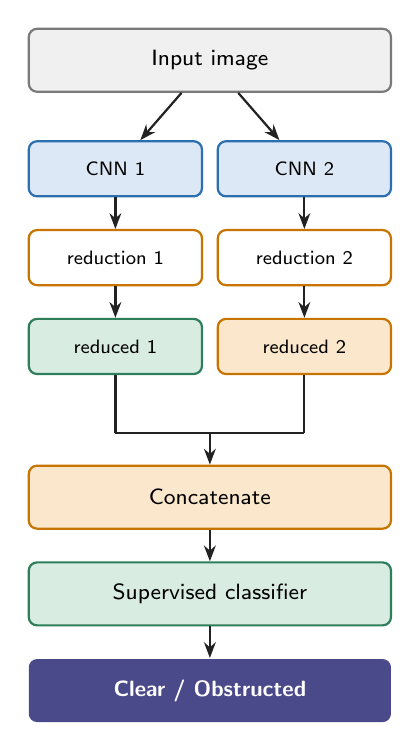
\begin{tikzpicture}[node distance=4mm]
\node[vw, draw=cInk!60, fill=gray!12] (im){Input image};
\node[vb, draw=cExtract, fill=cExtractL, below=6mm of im, xshift=-12mm] (c1){CNN 1};
\node[vb, draw=cExtract, fill=cExtractL, below=6mm of im, xshift=12mm] (c2){CNN 2};
\node[vb, draw=cReduce, fill=white, below=4mm of c1] (r1){reduction 1};
\node[vb, draw=cReduce, fill=white, below=4mm of c2] (r2){reduction 2};
\node[vb, draw=cClass, fill=cClassL, below=4mm of r1] (v1){reduced 1};
\node[vb, draw=cReduce, fill=cReduceL, below=4mm of r2] (v2){reduced 2};
\node[vw, draw=cReduce, fill=cReduceL, below=6mm of im |- v1, yshift=-9mm] (cc){Concatenate};
\node[vw, draw=cClass, fill=cClassL, below=of cc] (clf){Supervised classifier};
\node[vw, fill=cOut, text=white, font=\footnotesize\bfseries, below=of clf] (o){Clear / Obstructed};
\draw[vflow](im)--(c1);\draw[vflow](im)--(c2);
\draw[vflow](c1)--(r1);\draw[vflow](c2)--(r2);
\draw[vflow](r1)--(v1);\draw[vflow](r2)--(v2);
\coordinate (by) at ([yshift=4mm]cc.north);
\draw[line width=0.8pt,draw=cInk] (v1.south) -- (v1.south|-by);
\draw[line width=0.8pt,draw=cInk] (v2.south) -- (v2.south|-by);
\draw[line width=0.8pt,draw=cInk] (v1.south|-by) -- (v2.south|-by);
\draw[vflow] (cc.north|-by) -- (cc.north);
\draw[vflow](cc)--(clf);\draw[vflow](clf)--(o);
\end{tikzpicture}
\end{document}
